\chapter{Hardware Komponenten}\label{Komponente}

In diesem Kapitel werden die f"ur das gesamtsystem benutzten Har hinsichtlicht ihrer funktionsweise und Ansteuerung in Einzelnen erl"autert. 

\section{STM32L4 Discovery Kit}\label{LoRa}

Das STM32L4 Discovery Kit ist ein IoT Knoten, womit ein Benutzer Anwendungen mit direkter Verbindung zu einem oder mehreren Cloud-Servern entwickeln kann.
Dieses Discovery Kit erm\"oglicht eine Vielzahl von Anwendungen, indem es eine Multikink-Kommunikation (Bluetooth Low Energie) mit geringem Stromverbrauch  Multiway-Erkennung der Umwelt erm"oglicht (Siehe Abbildung \ref{Node}).

Das STM32L4 hat einen eingebetteten ST-LINK Debugger/Programmierer, eingebettete Sensoren und viele andere Features, die in dem Datenblatt \cite{B-L475E-IOT01A} erl"autert zu finden sind. Genau wegen der Vielfalt an Eingenschaften wurde dieses Board ausgew"ahlt. Man braucht kein Breadbord im Vergleich zu dem Arduino oder dem Raspberry-Pi, um die Sensoren mit den Schnittstellen (USART, SPI oder I2C) des Mikrocontrollers zu verbinden. Noch dazu eignet sich dieses Discovery Kit f"ur ein LoRa-Modul von STMicroelectronics, da Arduino-Verbinder vorhanden sind. Dazu ist nur das LoRa-Modul in dieser Verbinder stecken. 

\begin{figure}[h]
	\centering
	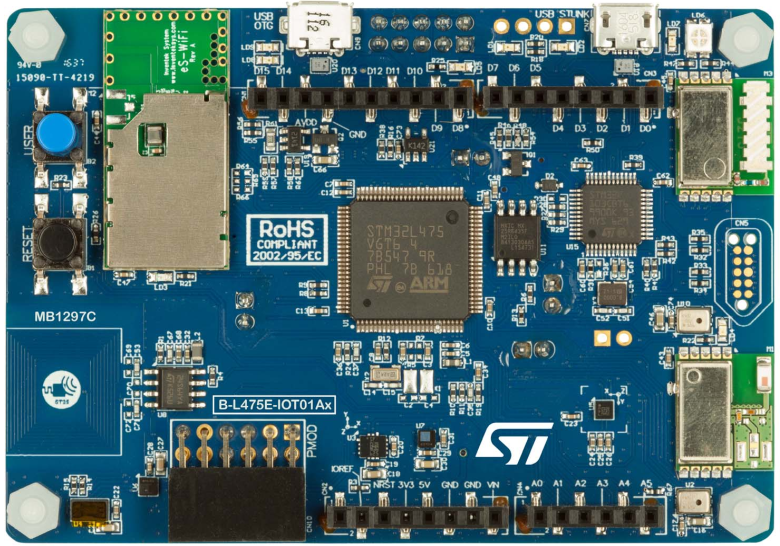
\includegraphics[width=9.5cm]{source/images/Board}
	\caption{B-L475E-IOT01A Discovery kit \cite{B-L475E-IOT01A}}\label{Node}
\end{figure}

\vspace{3cm}

F"ur diese Arbeit werden wir uns auf zwei Sensoren beschr"anken. Erstmal den HTS221\cite{HTS221} Temperatur- und Feuchtigkeitssensor und dann den LSM6DSK 3D-Gyroscope und 3D-Beschleunigungssensor \cite{LSM6DSL}. Diese Daten werden erfasst und drahtlos an den LoRaWAN-Server "ubertragen. Die folgenden Unterkapitel beschreiben, wie diese Sensoren funktionieren und erkl"aren, wie sie anzusteuern sind, damit die erhaltenen Daten im Rahmen der geforderten Toleranzen der Realit"at entsprechen. Laut dem Datenblatt ist mit einer Temperaturgenauigkeit von \textpm 0.5\textdegree{}c und einer Feuchtigkeitsgenauigkeit von \textpm 3.5\%   zu rechnen. 

\subsection {HTS221 Temperatursensor- und Feuchtigkeitssensor}\label{Temp}
In diesem Unterkapitel wird der HTS221 Temperatur- und Feuchtigkeitssensor beschrieben und erkl"art wie die Temperatur und die Feuchtigkeit zu ermitteln sind.

Der HTS221 Sensor misst die relative Feuchtigkeit(H) und die Temperatur (T) und speichert die Daten (16-Bits von Datentyp Integer) als Zweierkomplement. Diese Daten k"onnen "uber I2C- oder SPI-Schnittstelle gelesen werden. Die gespeicherte Daten sind Rohdaten, die am Ausgang von dem Analog-Digital-Converter (ADC) verf"ugbar sind (Siehe Abbildung \ref{HT_sensor}). Um die Temperatur in \textdegree{}c und die relative Feuchtigkeit in \% zu bekommen, muss man die Daten aus den Registern auslesen und mit Hilfe der Formel \ref{HumFormel} und \ref{TempFormel} die richtigen Werten herausfinden.

\begin{figure}[h]
	\centering
	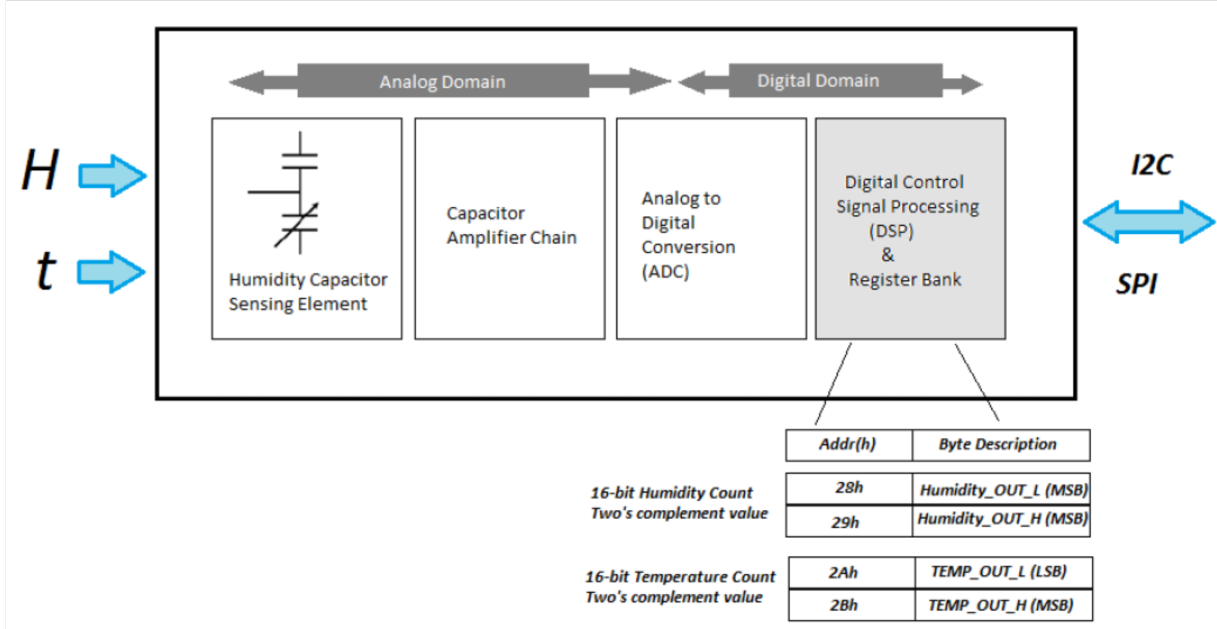
\includegraphics[width=14cm]{source/images/HTS221_sensor}
	\caption{Humidity sensor analog-to-digital flow \cite{HTS221}}\label{HT_sensor}
\end{figure}

\subsubsection{Feuchtigkeit ermitteln}

An dieser Stelle wird erkl"art wie die Feuchtigkeit von dem Sensor ermittelt wird.
Der HTS221 Sensor speichert den Feuchtigkeitswert in Rohz"alungen in zwei 8-Bit-Registern:
\begin{itemize}
	\item H\_OUT\_H (0x29) (H"ochstwertige Bits)
	\item H\_OUT\_L (0x28) (Niedrigswertige Bits)
\end{itemize}

Die zwei Bytes werden verkettet, um ein Zweierkomplement dargestelltes 16-Bit Wort zu bilden. Der relative Feuchtigkeitswert muss durch lineare Interpolation
der Register (HUMIDITY\_OUT\_H \& HUMIDITY\_OUT\_L) mit den Kalibrierregistern berechnet werden.

Der HTS221 Sensor ist bei der Herstellung schon kalibriert und die erforderlichen Koeffizienten sind ADC 16-Bit-Werte, die in den internen Register des Sensors zu lesen sind. Eine weitere Kalibrierung durch den Benutzer ist nicht erforderlich.

Die Tabelle \ref{tab:Reg_H} stellt die Register dar, in dem die Kalibrierwerte zur Ermittlung der relativen Feuchtigkeit gespeichert sind.

\begin{center}
	\begin{table}[htbp] 
		\centering 
		\Large
	%	\footnote{(u16) 16Bit-Wert ohne Vorzeichen, (s16) 16-Bit-wert mit Vorzeichen}
		\begin{tabular}{l|c|r}
			\textbf{Variable} & 	\textbf{Adresse} & \textbf{Format}\footnotemark\\
			\hline
			H0\_rH\_x2	& 0x30	& u(8) \\
			\hline
			H1\_rH\_x2	& 0x31	& u(8)\\
			\hline
			H0\_TO\_OUT\_H & 0x36	& s(16)\\
			\hline
			H0\_TO\_OUT\_L 	& 0x37  & s(16)\\
			\hline
			H1\_TO\_OUT\_H	& 0x3A	& s(16)\\
			\hline
			H1\_TO\_OUT\_L 	& 0x3B  & s(16)\
		\end{tabular} 
		\caption{Kalibrierregister f"ur relative Feuchtigkeit} 
		\label{tab:Reg_H} 
		 
	\end{table}
\end{center}
\footnotetext{(u8) 16Bit-Wert ohne Vorzeichen, (s16) 16Bit-Wert mit Vorzeichen}

Nun wissen wir welche Register zu lesen sind, damit die relative Feuchtigkeit mithilfe der Interpolation berechnet wird. Die folgenden Schritten m"ussen vor der Berechnung durchgef"uhrt werden:

\begin{itemize}
	\item Werte von H0\_rH\_x2 und H1\_rH\_x2 aus Registern 0x30 und 0x31 lesen 
	\item H0\_rH\_x2 und H1\_rH\_x2 durch zwei teilen
	\item Werte von H0\_TO\_OUT aus Registern 0x36 und 0x37 lesen 
	\item Werte von H1\_TO\_OUT aus Registern 0x3A und 0x3B lesen
	\item Rohdate von H\_T\_OUT aus Registern 0x28 und 0x29 lesen
\end{itemize}

Nachdem diese Register gelesen wurden, kann nun die Berechnung der relative Feuchtigkeit erfolgen.

\begin{figure}[h]
	\centering
	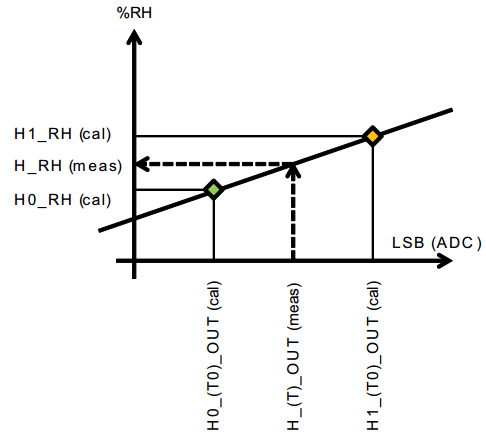
\includegraphics[width=9cm]{source/images/rH}
	\caption{Linear interpolation to convert LSB to \%RH \cite{HTS221}}\label{graph:rH}
\end{figure}

\vspace{3cm}
Aus Abbildung \ref{graph:rH} bekommt man mit Interpolation die folgende Formel \cite{HTS221}:

\begin{center}
	\[
	RH\% = \frac{((H1\_rH - H0\_rH) . (H\_T\_OUT - H0\_T0\_OUT))}{(H1\_T0\_OUT - H1\_T0\_OUT) } + H0\_rH  
	\]\label{HumFormel}
\end{center}


\subsubsection{Temperatur ermitteln}
Der HTS221 Sensor speichert die Temperaturwerten in Rohz"alungen in zwei 8-Bit-Registern:

\begin{itemize}
	\item T\_OUT\_H (0x2A) (H"ochstwertige Bits)
	\item T\_OUT\_L (0x2B) (Niedrigswertige Bits)
\end{itemize}

Die zwei Bytes werden verkettet, um ein Zweierkomplement dargestelltes 16-Bit Wort zu bilden. Die Polarit"at wird duch den h"ochstwertigen Bit vom T\_OUT\_H Register bekannt gegeben.

\begin{itemize}
	\item Ist dieser Bit 0, die gelesene Temperatur ist positiv.
	\item Ist dieser Bit 1, die gelesene temperatur ist negativ. In diesem fall ist der Zweierkomplement des gesamten Wort zu bilden, um den richtigen Wert zu bekommen.
\end{itemize}

\vspace{2cm}
Auch hier ist die Temperatur durch lineare Interpolation von den Kalibrierregistern und den Registern T\_OUT\_H und T\_OUT\_H in Zweierkomplement zu berechnen.

Die Tabelle \ref{tab:Reg_T} stellt diese Kalibrierregister dar.

\begin{center}
	\begin{table}[htbp] 
		\centering 
		\Large
		%	\footnote{(u16) 16Bit-Wert ohne Vorzeichen, (s16) 16-Bit-wert mit Vorzeichen}
		\begin{tabular}{l|c|r}
			\textbf{Variable} & 	\textbf{Adresse} & \textbf{Format} \\
			\hline
			T0\_degC\_x8	& 0x32	& u(8) \\
			\hline
			T1\_degC\_x8	& 0x33	& u(8)\\
			\hline
			T1/TOmsb & 0x35	& (u2),(u2)\\
			\hline
			T0\_OUT\_H 	& 0x3D  & s(16)\\
			\hline
			T0\_OUT\_L 	& 0x3C  & s(16)\\
			\hline
			T1\_OUT\_H	& 0x3F	& s(16)\\
			\hline
			T1\_OUT\_L 	& 0x3E  & s(16)\
		\end{tabular} 
		\caption{Kalibrierregister zur Temperaturermitllung} 
		\label{tab:Reg_T} 
		
	\end{table}
\end{center}

Da die Kalibrierregister vom Hersteller mit den korrekten Werten versehen werden, werden wir nun diese Register lesen und mithilfe der gelesenen Werten die Temperatur ermitteln. Bevor man die Temperatur mit linearer Interpolation berechnet, sind die folgenden Schritten erstmal erforderlich.

\begin{itemize}
	\item Die Koeffiziente T0\_degC\_x8 und T1\_degC\_x8 aus den Registern 0x32 und 0x33 lesen
	\item Die Werte von T0\_degC\_x8 und T1\_degC\_x8 durch 8 divisiren, um die Koeffiziente T0\_degC und T1\_degC zu bekommen.
	\item Die h"ochstwertige Bits von T1\_degC(T1.9 und T1.8) und T0\_degC(T0.9 und T0.8) aus dem Register 0x35 lesen. Diese Werte an den im Schritt 2 ermittelten Werten verketten, damit T0\_degC und T1\_degC vollst"andig werden.
	\item Der Wert von T0\_OUT aus den Registern 0x3C und 0x3D lesen.
	\item Der Wert von T1\_OUT aus den Registern 0x3E und 0x3F lesen.
	\item Der Wert von T\_OUT aus den Registern 0x2A und 0x2B lesen.
	 	
\end{itemize}

Nachdem diese Kallibrierregister gelesen wurden, kann man mittels linearer Interpolation die Temperatur in \textdegree{}c berechnen.

\begin{figure}[h]
	\centering
	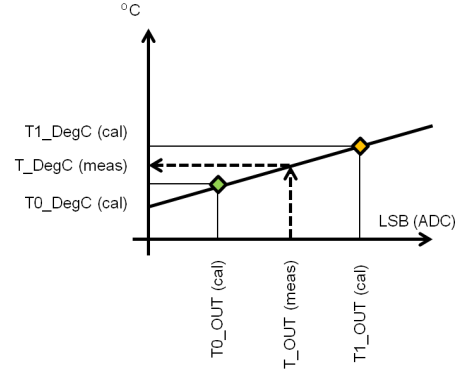
\includegraphics[width=9cm]{source/images/Temp}
	\caption{Linear interpolation to convert LSB to \textdegree{}c \cite{HTS221}}\label{graph:T}
\end{figure}

\vspace{3cm}

Abbildung \ref{graph:T} zeigt der Graph woraus die lineare Interpolation stammt. Die folgende Formel wurde sogar daraus hergeleitet.

\begin{center}
	\[
	T[\textdegree{}c] = \frac{((T1\_degC - T0\_degC) . (T\_OUT - T0\_OUT))}{(T1\_OUT - T0\_OUT) } + T0\_degC  
	\]\label{TempFormel}
\end{center}

 Da die Kalibrierwerten zur Berechnung der Temperatur und der relativen Feuchtigkeit bei der Herstellung des Bausteins vorab festgesetzt sind, soll man die Kalibrierregister bei der Programmierung nur ein mal auslesen. Dies erspart den Rechenaufwand des Mikrocontrollers.
 
\subsection{LSM6DSL 3D Gyroskope und 3D Beschleunigungssensor}\label{Acc/Gy}

Dieses Unterkapitel berichtet von dem LSM6DSL 3D-Gyroskope und 3D-Beschleuni- gungssensor. Hier ist zu entnehmen, wie die X-,Y-, und Z-Koordinaten des Sensoren zu ermitteln sind und wie der Sensor abh"angig vom Zweck skaliert werden kann.
 

Der LSM6DSL ist ein digitaler 3D-Beschleunigungsmesser und ein 3D-Gyroskopsystem mit einer digitalen seriellen I2C/SPI Schnittstelle mit einer leistung von 0.65mA im kombinierten Hochleistungsmodus.
Das Ger"at verf"ugt "uber einen von Benutzer w"ahlbaren dynamischen Beschleunigungsbereich von \textpm 2 \textbar \textpm 4 \textbar \textpm 8 \textbar \textpm 16g (g is gleich 9,81m/s) und einen Winkelgeschwindigkeitsbereich von \textpm 125 \textbar \textpm 250 \textbar \textpm 500 \textbar \textpm 1000 \textbar \textpm 2000dps (Degrees per second).
 
Das extrem geringe Gr"o\ss{}e und das geringe Gewicht des SMD-Packets machen den LSM6DSL zu einer idealen Wahl f"ur tragbare Anwendungen wie Smartphones, IoT-verbundene Ger"ate und andere Anwendungen, bei der reduzierte Paketgr"o\ss{}e und -gewicht erforderlich sind.  

Der LSM6DSL bietet drei m"ogliche Betriebskonfiguration:
\begin{itemize}
	\item nur Beschleunigungsmesser aktiv und Gyroskope inaktiv
	\item nur Gyroskope aktiv und Beschleunigungsmesser inaktiv
	\item beide aktiv mit unabh"angigem Output Data Rate (ODR) 
\end{itemize}

Der Beschleunigungsmesser und der Gyroskop k"onnen unabh"angig voneinander konfiguriert werden unteranderem: Power-down, Low-Power, Normal- und High- performance Modus. Um den Stromverbrauch des Sensors zu reduzieren, kann der Gyroskop in einem Ruhestand gesetzt werden.


Sobald das Ger"at mit Strom versorgt wird, werden die Kalibriekoeffizienten vom eingebettetem Flash-Speicher zu den internen Registers. Dieser Vorgang dauert ungef"ahr 15 milisekunden. Nach dieser Zeit fallen der Beschleunigungsmesser und der Gyroskop im Power-Down Modus. Durch der CTRL1\_XL bzw. CTRL2\_G register k"onnen die Ger"ate geweckt werben, indem man das Betriebmodus ausw"ahlt.

Wenn die Daten verf"ugbar sind, wird eine Unterbrechung (Interrupt demn"achst) ausgel"ost, wenn der entsprechende Byte vom Beschleunigungsmesser bzw. vom Gyroskop in dem INT1\_CTRL Register geschrieben wurde. Das vorhandensein der Daten kann nun mit Hilfe des Statusregister abgefragt werden. Das XLDA-Bit wird auf 1 gesetzt, wenn am Ausgang des Beschleunigungsmesser ein neuer Datensatz verf"ugbar ist. Das GDS-Bit wird suf 1 gesetzt, wenn am Gyroskopausgang ein neuer Datensatz verf"ugbar ist.

\begin{figure}[h]
	\centering
	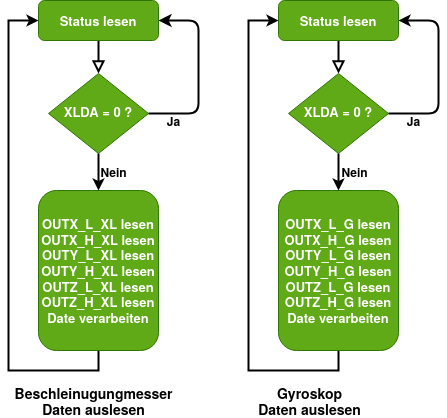
\includegraphics[width=8cm]{source/images/Gy_Acc_data}
	\caption{Flu\ss{}diagram zur Datenermitlung}\label{Gy_Acc_data}
\end{figure}

Das Abbildung \ref{Gy_Acc_data} ist der Flu\ss{}diagram zur ermitllung der Achsen- und Winkelver"anderungen des Beschleunigungsmesser und des Gyroskop.

Wie oben schon erl"autert, kann das Ger"at so eingestellet werden, dass ein neuer Satz von Messdaten durch ein Signal erkennbar wird. Das XLDA-Bit von dem STATUS\_REG-Register wird auf 1 gesetzt, wenn Daten aus dem Beschleunigungsmesser zum Lesen verf"ugbar sind. Das Signal kann durch den INT1-Pin angesteuert werden, indem  das INT1\_DRDY\_XL-Bit vom INT1\_CTRL-Register auf 1 gestezt wird. 

F"ur den Gyroskopsensor wird das GDA-Bit auf 1 gesetzt, wenn die Daten zum lesen verf"ugbar sind. Das Signal kann durch den INT1-Pin angesteuert werden, indem  das INT1\_DRDY\_G-Bit vom INT1\_CTRL-Register auf 1 gestezt wird. Die gemessenen Beschleunigungsdaten werden in OUTX\_H\_XL-, OUTX\_L\_XL-, OUTY\_H\_XL-, OUTY\_L\_-XL-, OUTZ\_H\_XL-, OUTZ\_L\_XL-Register gesendet. Die gemessenen Winkelgeschwindigkeitsdaten werden dagegen in OUTX\_H\_G-, OUTX\_L\_G-, OUTY\_H\_G-, OUTY\_L\_G-, OUTZ\_H\_G-, OUTZ\_L\_G-Register gesendet. Die vollst"andigen Ausgangsdaten f"ur die X-,Y- und Z-Achsen sind durch die Verkettung von OUTX\_H\_XL(G) und OUTX\_L\_-XL(G), OUTY\_H\_XL(G) und OUTY\_L\_XL(G), OUTZ\_H\_XL(G) und OUTZ\_L\_XL zu erhalten, wobei die Beschleunigungsdaten und die Winkelgeschwindigkeitsdaten als 16-Bit Werte dargestellt sind.

Mit dem LSM6DSL kann man den Inhalt des unteren und oberen Teils der Ausgangsdatenregister vertauschen, sodass die Darstellung entweder Big-Endian oder Little-Endian entspricht. Dies ist m"oglich, sofern man das BLE-Bit von dem CTRL3\_C-Register auf 0 (Little-Endian Standartm"a\ss{}ig) oder auf 1 (f"ur Big-Endian) 
Big-Endian bedeutet, dass der h"ochstwertige Byte des Datensatzes in der niedrigsten Speicherstelle gespeichert wird.
Little-Endian bedeutet, dass der niedrigswertige Byte des Datensatzes in der niedrigsten Speicherstelle gespeichert wird.


Im Unterkapitel \ref{Sensoren} weden die Funktionen zur Datenermittlung in der Programmiersprache C sowohl f"ur den HTS221 (Temperatur- und Feuchtigkeitssensor) als auch f"ur den LSM6DSL (3D-Beschleunigungsensor und 3D-Gyroskop) dargestellt und erkl"art wie die Kommunicationsschnitstelle (hier I2C) zu benutzen ist.


\vspace{5cm}
\section{LoRa Node: i-nucleo-lrwan1}\label{LoRa Modul}

Die im Kapitel \ref{Temp} ermittelten Sensordaten sollen laut der Aufgabestellung mit Hilfe eines drahtloses Protokol an einem Server versand werden. Um diese Daten drahtlos und auf eine lange Strecke zu "ubertragen, haben wir uns auf das LoRaWAN-Protokol entschieden. Die Gr"unde warum genau dieses Protokol ausgew"ahlt wurde, werden in diesem Kapitel genannt. Noch dazu wird nicht nur auf die Eigenschaften des benutzten LoRa-Modul eingegangen sondern auch auf den Unterschied von diesem Modul gegen"uber anderen Modulen, die auf dem Markt zu finden sind.   
 
 
\begin{figure}[h]
	\centering
	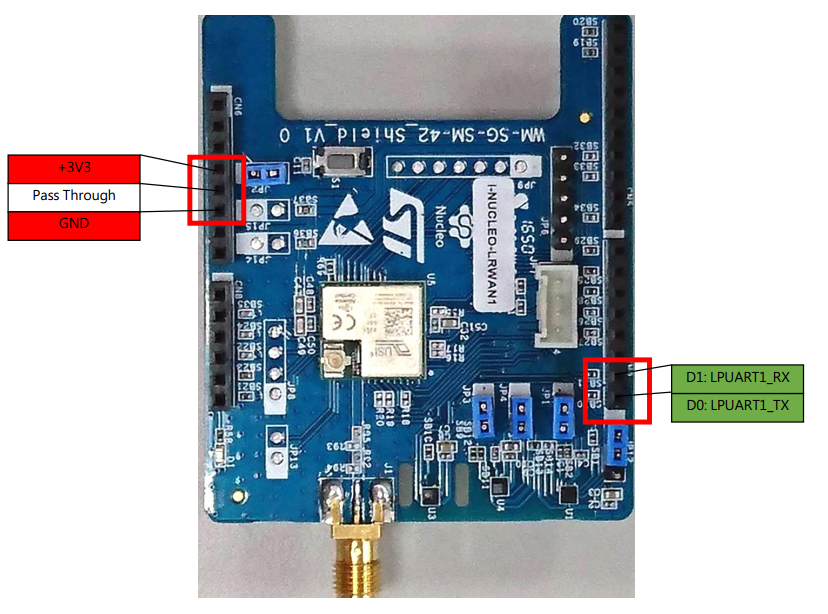
\includegraphics[width=14cm]{source/images/LoRa_mod}
	\caption{I-Nucleo-LRWAN1 \cite{LoRaMod}\label{graph:loraMod}}
\end{figure}

Abbildung \ref{graph:loraMod} zeigt das LoRa-Modul, das zur Daten"ubertragung verwendet ist. Diese Platine mit Arduino-Connectoren und mehr ist eine integrierte L"osung, die jedem erm"oglich Anwendungen mit der LoRa-Technologie zu entwickeln. Das I-Nucleo-LRWAN1 verf"ugt "uber den USI\textregistered\ LoRaWAN\texttrademark\ Technologiemodul f"ur konsteng"unstiges und stromsparendes Weitverkehrsnetz (LPWAN), welches mit einem eingebetteten Stapel von AT-Befehle (AT-Befehl beschreiben) mitgeliefert wird.
Dieses Board wurde ausgew"ahlt, weil es durch ein externes Board wie das Nucleo-L053 oder user B-L475E-IOT01A Discovery kit \ref{Node} "uber mehrere Schnittstellen wie LPUART, SPI oder I2C angesteuert werden kann. Noch dazu verf"ugt das I-Nucleo-LRWAN1 "uber die folgenden eingebetteten Sensoren.

\begin{itemize}
	\item ST Beschleunigungs- und Magnetosensor (LSM303AGR)
	\item ST relative Feuchtigkeits- und Temperatursensor (HTS221)
	\item ST Drucksensor (LPS22HB)
\end{itemize}

Im Vergleich zu anderen LoRa-Modulen, worauf keine Sensoren vorhanden sind, brau-cht man keine zus"atzliche Sensoren kaufen. Die Kommunikation mit einem anderen Mikrocontroller erfolgt einfach durch UART, man braucht nicht auf das integriete Radio-Modul zum Senden oder Empfangen von Daten und Befehle zu k"ummern. Das Bild \ref{graph:loraMod_intern} zeigt, dass das I-Nucleo-LRWAN1 mit einem STM32L0-Mikrocontroller versehen ist, der dazu zust"andig ist, die Kommunikation zwischen dem I-Nucleo-LRWAN1 und einem externen Mikrocontroller zu vereinfachen. Das SX1272-Chip ist das eigentliche LoRa-Radio-Modul, das die Daten oder die Befehle per Funk durch die Antenne an entweder einem Gateway (Router) oder einem anderen LoRa-Node  sendet. 

\begin{figure}[h]
	\centering
	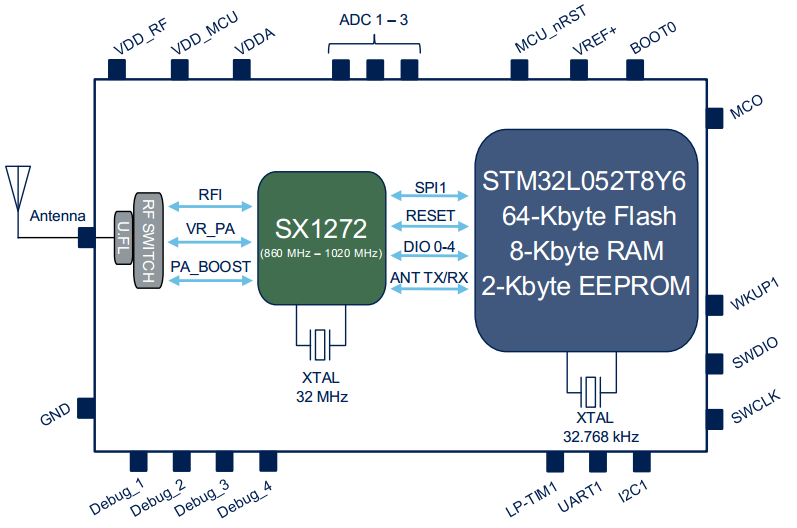
\includegraphics[width=14cm]{source/images/LoRa_Intern}
	\caption{I-Nucleo-LRWAN1 Architektur \cite{LoRaMod}\label{graph:loraMod_intern}}
\end{figure}



\subsection{LoRaWAN Protokol}\label{LoRaWAN_P}
\subsubsection{Aktivierung durch OTAA}
\subsubsection{Aktivierung durch ABP}
\subsection{AT Commandos}\label{AT}


\chapter{Gateway und LoRaWAN-Server}\label{G_S}

\section{Gateway}\label{Gateway}
\subsection{Was ist das Lora packet forwarder}
\section{Einstellung des LoRaWAN-Servers}\label{server}
\section{MQTT brocker zur Daten"ubertragung}


\chapter{Software-Entwicklung}\label{Soft-Ent}
\section{Entwicklungsumgebung}
\subsection{Eclipse}
\subsection{Libopencm3 Bibliotek installieren}
\section{Sensoren Auslesen} \label{Sensoren}
\section{LoRa Commandos senden}
